\chapter{Results}
\label{results}

In this section I present the results of the three experiments (Initial Curiousity, Exploiting Information, and Long-Term Success) detailed in \cref{sec:simulations}. For each experiment the analyses are available for all four agents (BFE, GFE, Context-BFE, and Context-GFE) with two parameter sweeps (\(\alpha \in [0.0, 0.1, \dots, 1.0]\), and \(c \in [0, 1, \dots, 10]\)) each. This leads to visualizations that contain four heatmaps (for the four agents) where the two axes represent the two parameter sweeps (over \(\alpha\) and \(c\)). The result for a specific constellation of agent type, \(\alpha\) value, and \(c\) value is then given in the specific cell of the heatmap. The heatmaps assign brighter and darker colors to higher and lower values respectively. For the following it is useful to recall what the different agents types, \(\alpha\) values, and \(c\) values refer to.

Both BFE Agent and Context-BFE Agent are not curious and do not seek out information in the environment to reduce uncertainties in their generative models. Conversely, the GFE Agent and Context-GFE Agent do exactly that, i.e., they are indeed curious and are driven to reduce uncertainties.
Orthogonally to the two properties "curious" and "non-curious", the agents can also be categorized as having a context state or not having a context state. Following this, both Context-BFE Agent and Context-GFE Agent possess a context state, which in the case of the Context-GFE Agent is subject to reducing its uncertainty as a result of the curiousity. Conversely, the BFE Agent and GFE Agent do not possess a context state and the curiousity of the GFE Agent then attempts to reduce uncertainty of the basic hidden state (all four agents possess hidden states as part of their generative models but two of them additionally have context states).

The \(\alpha\) values relate the T-Maze type (A or B) to the true reward location (left arm or right arm). Values close to \(1.0\) strongly relate T-Maze type A with a reward in the left arm (and type B with the right arm). In contrast, values close to \(0.0\) relate T-Maze type A with a reward in the right arm (and type B with the left arm). Values near \(0.5\) implicate that knowing about the type of T-Maze does (almost) not yield any information about the true reward location.

The \(c\) values are also parameters of the agents' generative models. They define how much the agent is actually interested in receiving (observing) the reward. To give an intuition for the values, \(c=0\) means it wants to receive the reward in \(25\%\) of the cases, \(c=1\) means it wants it in \(\sim53.4\%\) of the cases, \(c=2\) means it wants it in \(\sim77.6\%\) of the cases, \(c=5\) means it wants it in \(\sim98.7\%\) of the cases, and \(c=10\) means it wants it in \(\sim100\%\) of the cases.


\section{Experiment 1: Initial Curiousity}

In this section I analyze the results of \cref{fig:19}. Here, the behavioral modes of all agents can be divided along two dimensions (not to be confused with the two axes in each plot): First, all agents are driven by a (varying) desire for observing the reward. Second, the curious agents also "want" to reduce uncertainty about hidden states (including context states) of their generative models. Both behavioral drives are investigated in the following.
The values in the heatmaps' cells (\cref{fig:19}) give the inferred probabilities of executing the action in timestep \(t=0\) that moves the agent to the cue location in the T-Maze. The values are not based on emperical measurements but directly represent the agents' beliefs about their actions.

\begin{figure}[htbp]
    \centering
    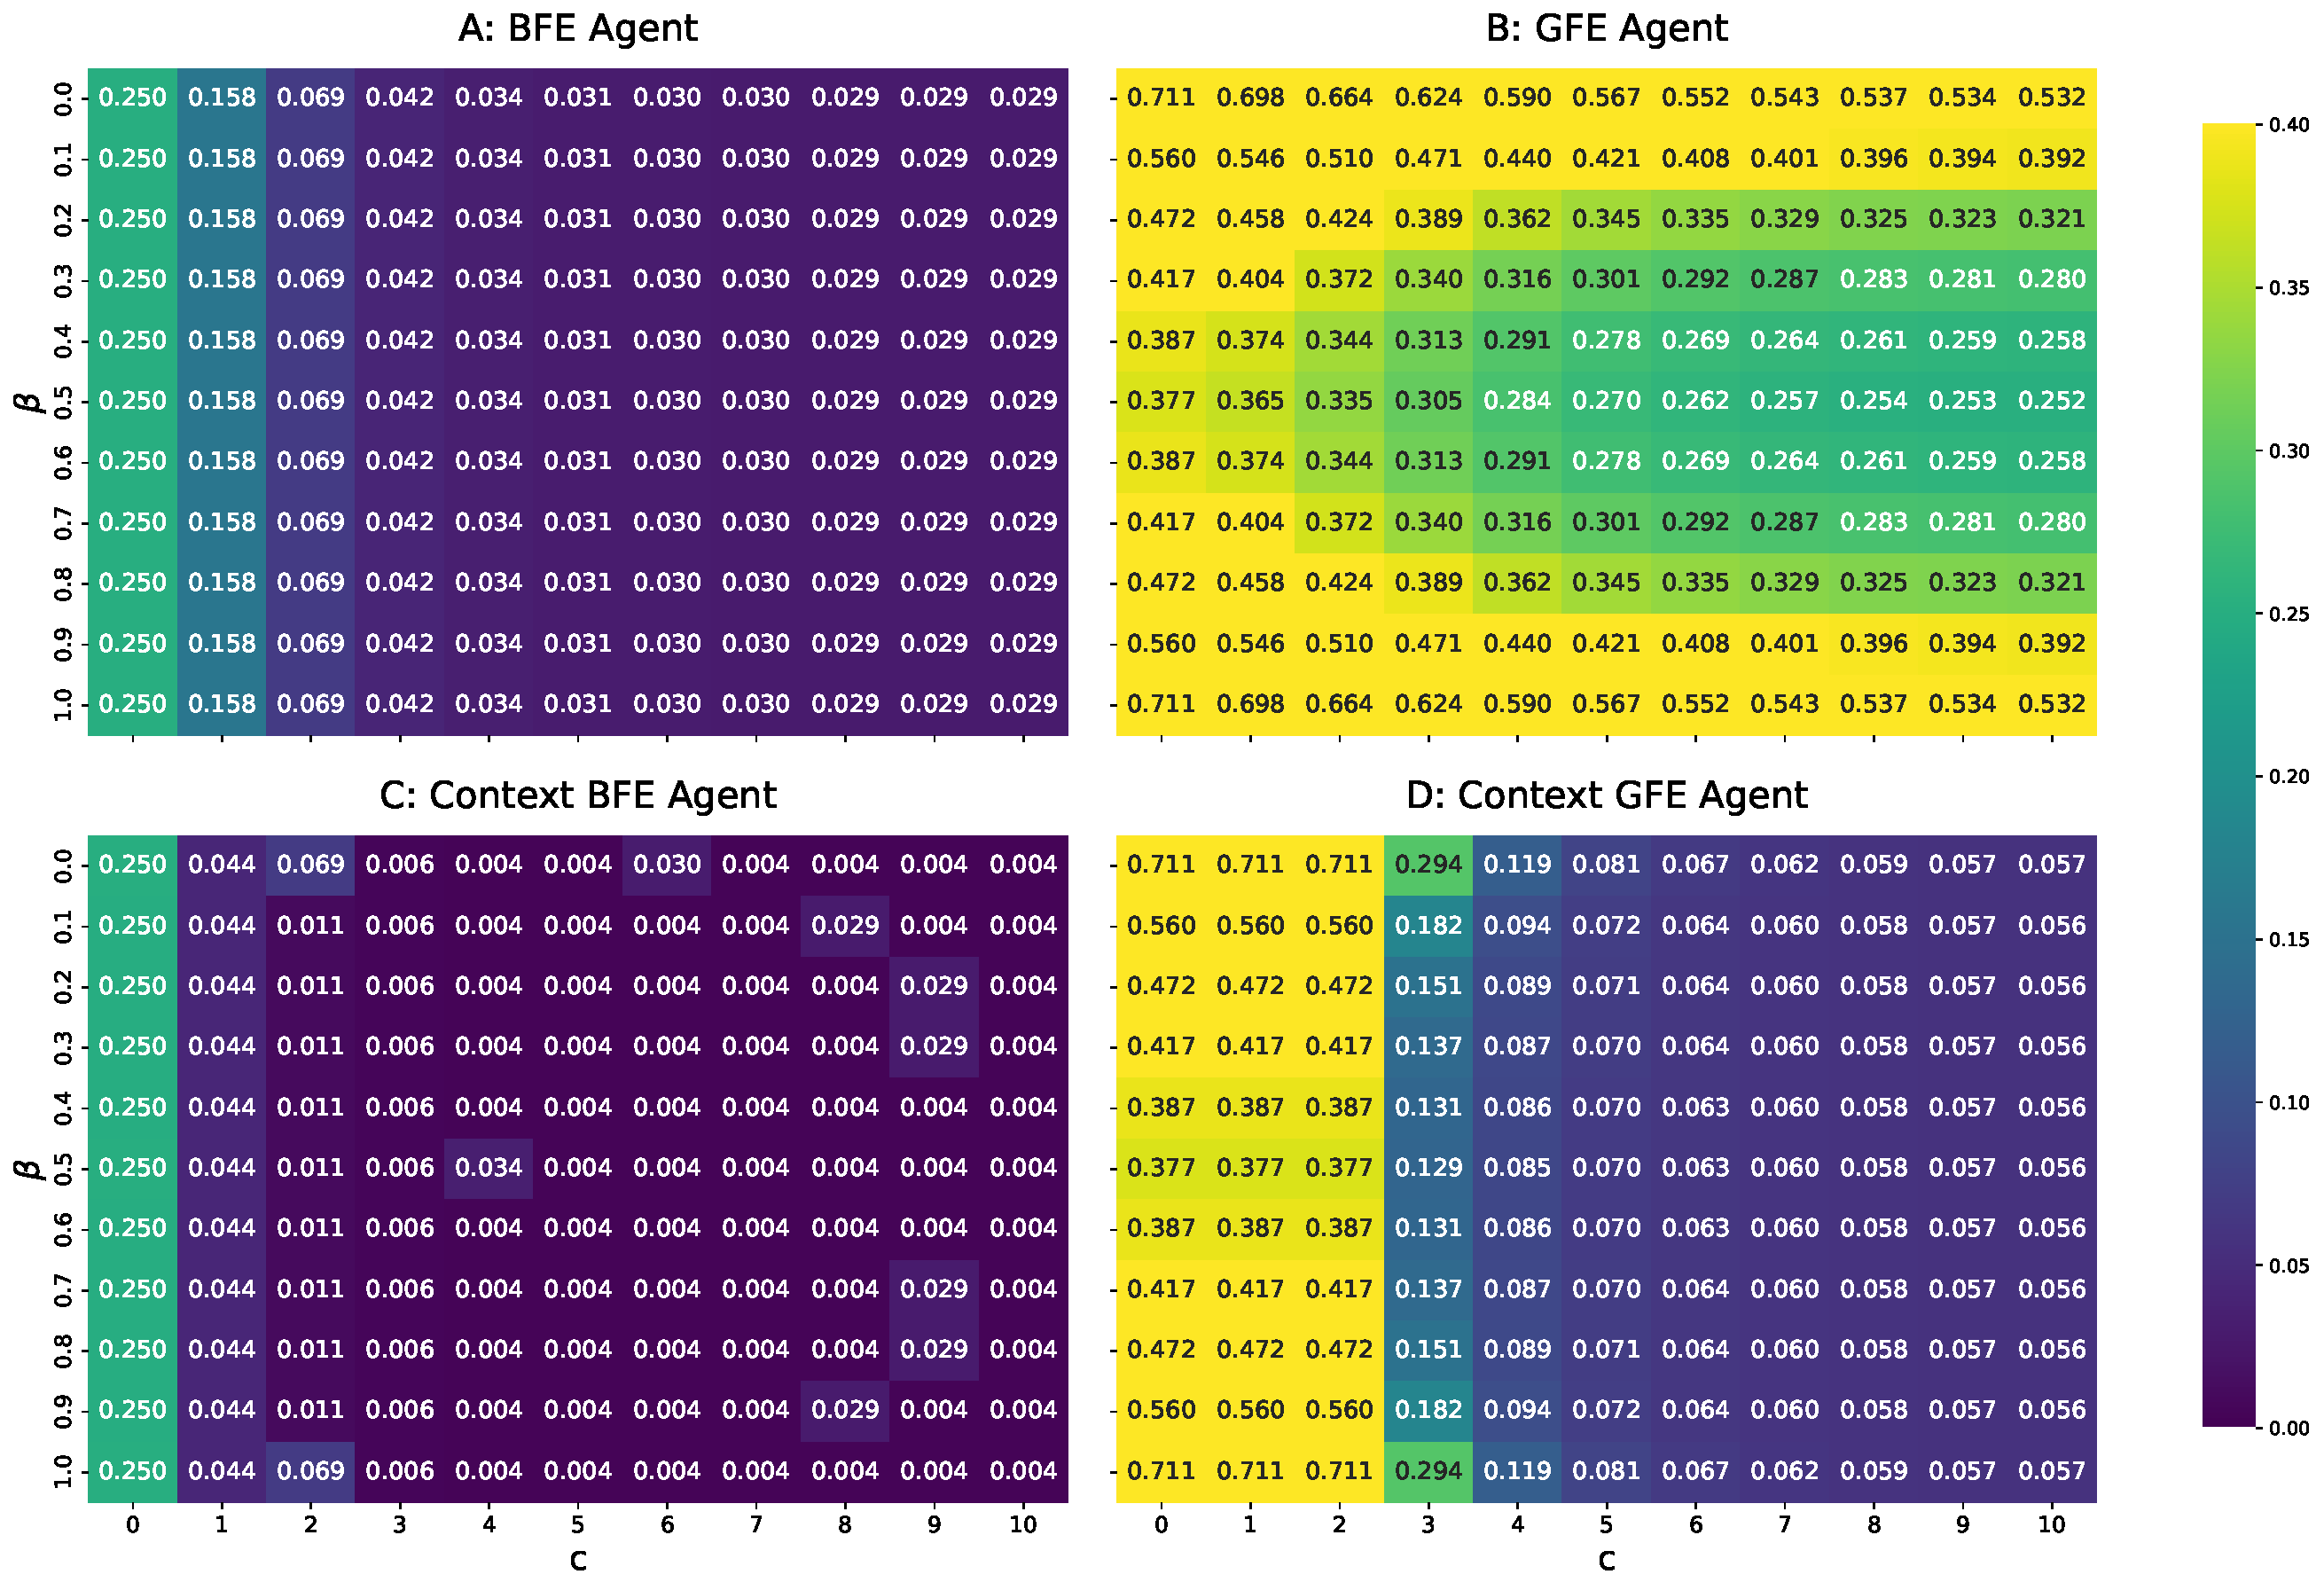
\includegraphics[width=\textwidth]{figures/simulation_1_cue.pdf}
    \caption{Inferred probabilities of executing an action in timestep \(t=0\) that moves the agent to the cue for the four agents (BFE, GFE, Context-BFE, and Context-GFE) with differing \(\alpha\)- and \(c\) values.}
    \label{fig:19}
\end{figure}

\subsubsection{Desire for observing the Reward}

All agents know the reward is located in one of the two arms in the T-Maze but certaintly not at the two remaining locations (start and cue). When the agent has a stronger preference for the reward (higher \(c\) value) then it is also more likely to directly move to one of two arms and effectively gambles for the reward (there is a \(50\,\%\) chance of observing the reward). In return the probabilities of performing an alternative action (e.g., "move to cue", or "move (stay) at start") become smaller. This consequence is evident in each agent type, where the probabilities of moving to the cue become smaller for larger \(c\) values.

\subsubsection{Desire for reducing Uncertainty}

The drive for reducing uncertainty about hidden states (including context states) is only evident in the curious agents. In the following, I explain the curiousity mechanism and how it relates to the results of the agents. High uncertainty levels of hidden states in the generative model relates to the agent's assumption that some hidden causes of observations in the environment are not clear, meaning the agent assigns similar (highly entropic) probabilities to the different possible causes. In this simulation, the hidden causes of observations consist of the four T-Maze fields (left arm, right arm, start, and cue) and the two T-Maze types (type A, and type B). Regarding the fields, they are immediately disclosed at each observation, e.g., when the agent is at the start it immediately knows (through the observation) that it is at the start field. In the case of the T-Maze types observations do not regularly reveal the type of the maze. This situation is mirrored in the agents' belief distributions about hidden states where the states concerning the T-Maze type initially are maximally uncertain, i.e., both possibilities (type A and type B) have equal (highly entropic) probabilities \(p=0.5\). The curiousity mechanism then aims at reducing this uncertainty (entropy). This is achieved by selecting actions that are expected to lead to observations that are informative about this hidden state. This requires further clarification: Observations can only be informative about hidden states when the agent has a model of the relation between that hidden state and possible observations, i.e, this relation must not be random. This circumstance can directly be exploited by the curious agent by moving to the cue location. There it receives an observation for which the agent possesses a deterministic model how this observation relates to the T-Maze type (one possible observation leads to \(p=1.0\) for type A and the other possible observation leads to \(p=1.0\) for type B). Besides directly moving to the cue location, there is a second option. The agent could also directly move to one of the two arms and thus observes the reward or no reward. This observation is also related to the T-Maze type but not deterministically but through the parameter \(\alpha\). This second option is only useful when \(\alpha \neq 0.5\), i.e, when there is a non-random relation between the observation and the T-Maze type. Moreover, more deterministic values like \(\alpha=0.0\) or \(\alpha=1.0\) makes this observation (reward) more useful, where it can then infer that the maze has type A in the former case and type B for the latter. In this situation, receiving no reward in an arm is also informative because the agent can then infer it is interacting with the opposite maze type. This circumstance becomes evident in the results of both curious agents. Both agents are driven by their curiousity and can only satisfy this "desire" by either going to the cue or moving to one of the arms--but only in the case when it knows what an observation at an arm means in relation to the hidden T-Maze type, i.e, when \(\alpha \neq 0.5\). In the most ambiguous case \(\alpha=0.5\), moving to an arm cannot satisfy the curiousity drive, i.e, it does not reduce uncertainty about the T-Maze type and thus the agent is then increasingly driven to reduce this uncertainty using the other option it still has: It instead moves to the cue. This trend is visible in the results of both curious agents where they initially move to the cue with highest probabilities (\(p=0.380\)) for \(\alpha\) values near \(0.5\). There is an additional aspect to consider: Though the agent has two options to satisfy its curiousity drive, one of them is potentially risky. When opting for moving to an arm to find out about the T-Maze type, it potentially misses out on the reward, which it strongly dislikes. In this way, curious agents balance the value of information with the value of receiving preferred observations, i.e., both motives have the same "currency".


\section{Experiment 2: Exploiting Information}

In this section I analyze the results of \cref{fig:20}. Again, the following behavioral analysis can be divided into two parts that first relate to all agents' drive to receive the reward, and second relate to the curious agents' drive to also seek information in the environment.
The values in the heatmaps' cells (\cref{fig:20}) give the inferred probabilities of moving to the arm in the T-Maze that is hinted by the cue to contain the reward (via the T-Maze type and parameter \(\alpha\). Again, the probabilities do not represent empirical measurements but beliefs of the agent that it will execute the action that moves it to the arm that should contain the reward according to the cue.

\begin{figure}[htb]
    \centering
    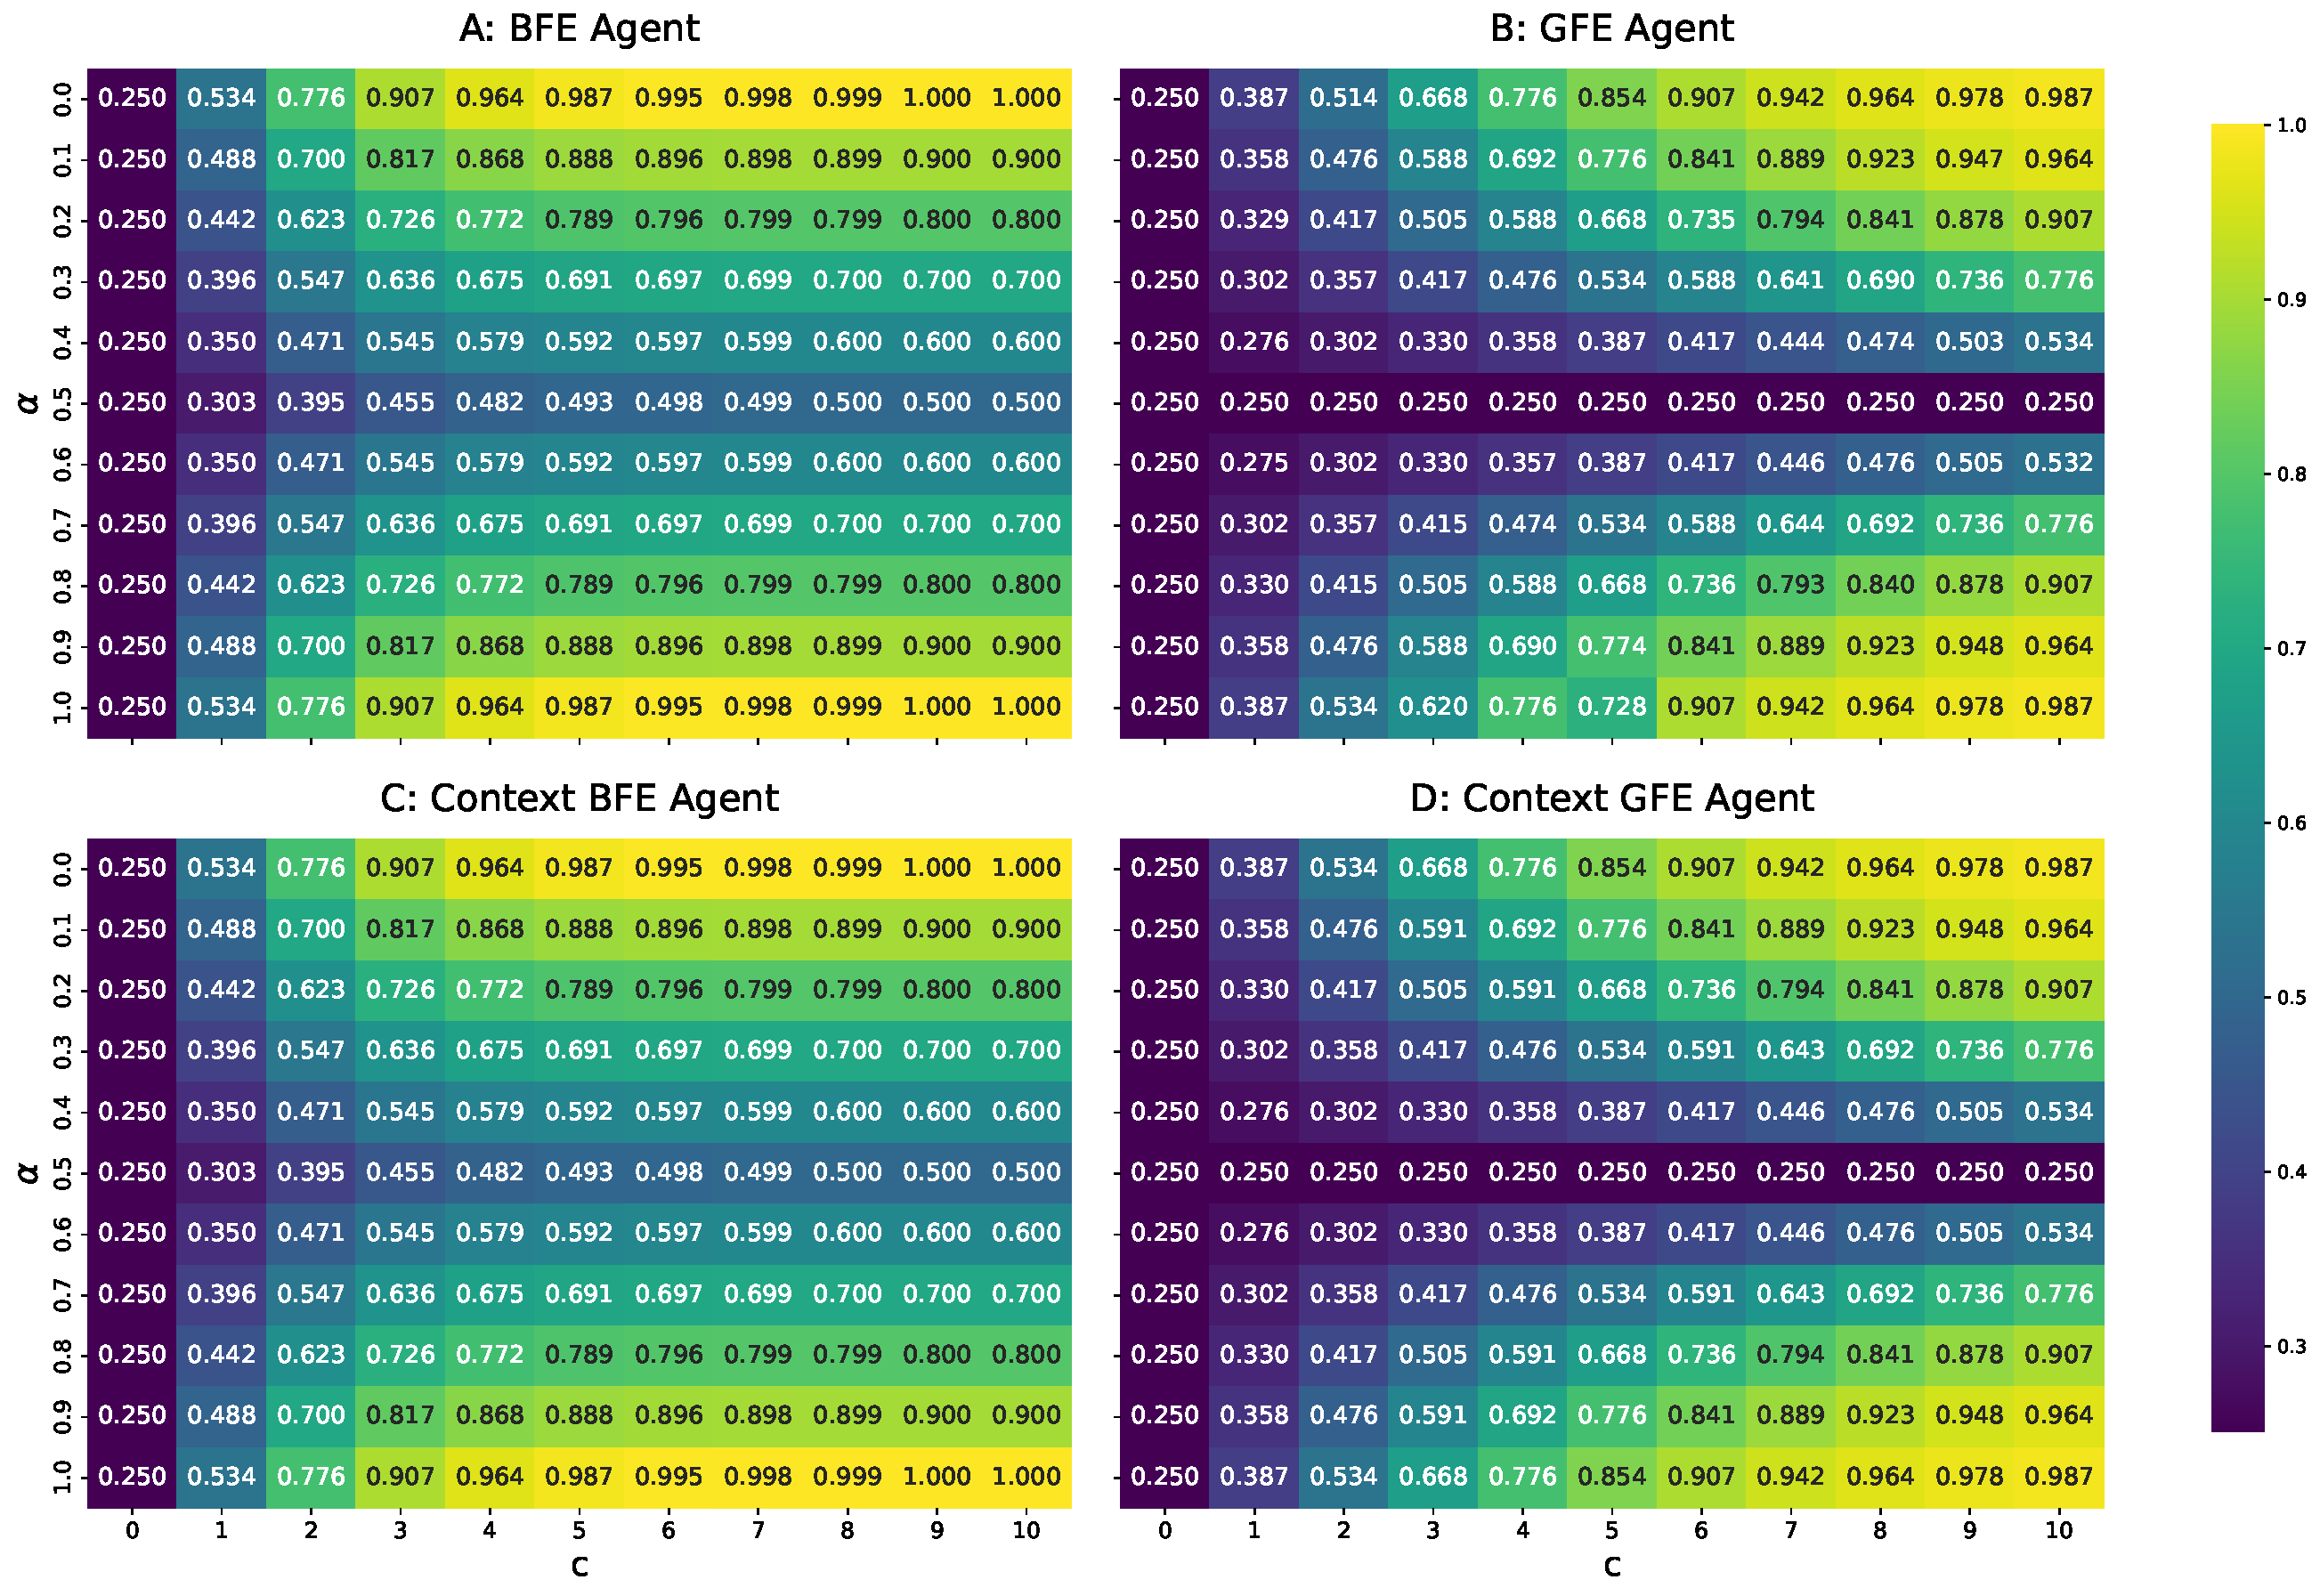
\includegraphics[width=\textwidth]{figures/simulation_2.pdf}
    \caption{Inferred probabilities of moving to the arm in the T-Maze that is hinted by the cue to contain the reward for the four agents (BFE, GFE, Context-BFE, and Context-GFE) with differing \(\alpha\)- and \(c\) values.}
    \label{fig:20}
\end{figure}

\subsubsection{Moving to the cued Reward Field}

All four agents show similar characteristics of moving to the arm field that is suggested by the cue. Specifically, the cue reveals the type of the T-Maze (type A or type B) and the agents can relate this information to the specific arm that is expected to contain the reward via the parameter \(\alpha\). Extreme \(\alpha\) values allow for a more certain prediction of the cue-containing arm field. This situation is evident in all four agents. The probabilities of moving to the arm that is suggested by the cue increase with more certain (extreme) \(\alpha\) values, i.e., the agents know there is a strong correlation between the T-Maze type and the location of the reward (left arm or right arm) and exploit this knowledge to find the reward.

Similarly, the \(c\) values describe the agents' preferences of observing the reward, where higher values lead to stronger preferences. This circumstance is visible in the results of all four agents where they all are more likely to move to the cued reward location with increasing \(c\) values, i.e, the more they "want" to receive the reward the more likely they exploit the information from the cue.

\subsubsection{Curious Agents still seek Information}

Both curious agents have similar results compared to the non-curious agents with subtle differences that seem to relate to their intrinsic drive to continue seeking information in the environment (even after receiving the cue). The curious agents yield lower probabilities of moving to the cued location for most \(\alpha\)- and \(c\) values, i.e., in these cases the curious agents assign more probability mass to other actions which indicates that these still reveal information that the agents seek. The few configurations of \(\alpha\)- and \(c\) values that have higher probabilities than the non-curious agents hint at the opposite: There the curious agents seem to assume information at these cued fields that can be exploited. These findings require further investigation.


\section{Experiment 3: Long-Term Success}


In this section I give the results of \cref{fig:21}. As for previous simulations the results show a behavioral divide between non-curious and curious agents. These are detailed in the following.
The values in the heatmaps' cells give the ratios of receiving the reward in timestep \(t=1\) or \(t=2\) over \(1000\) trials.

\begin{figure}[htbp]
    \centering
    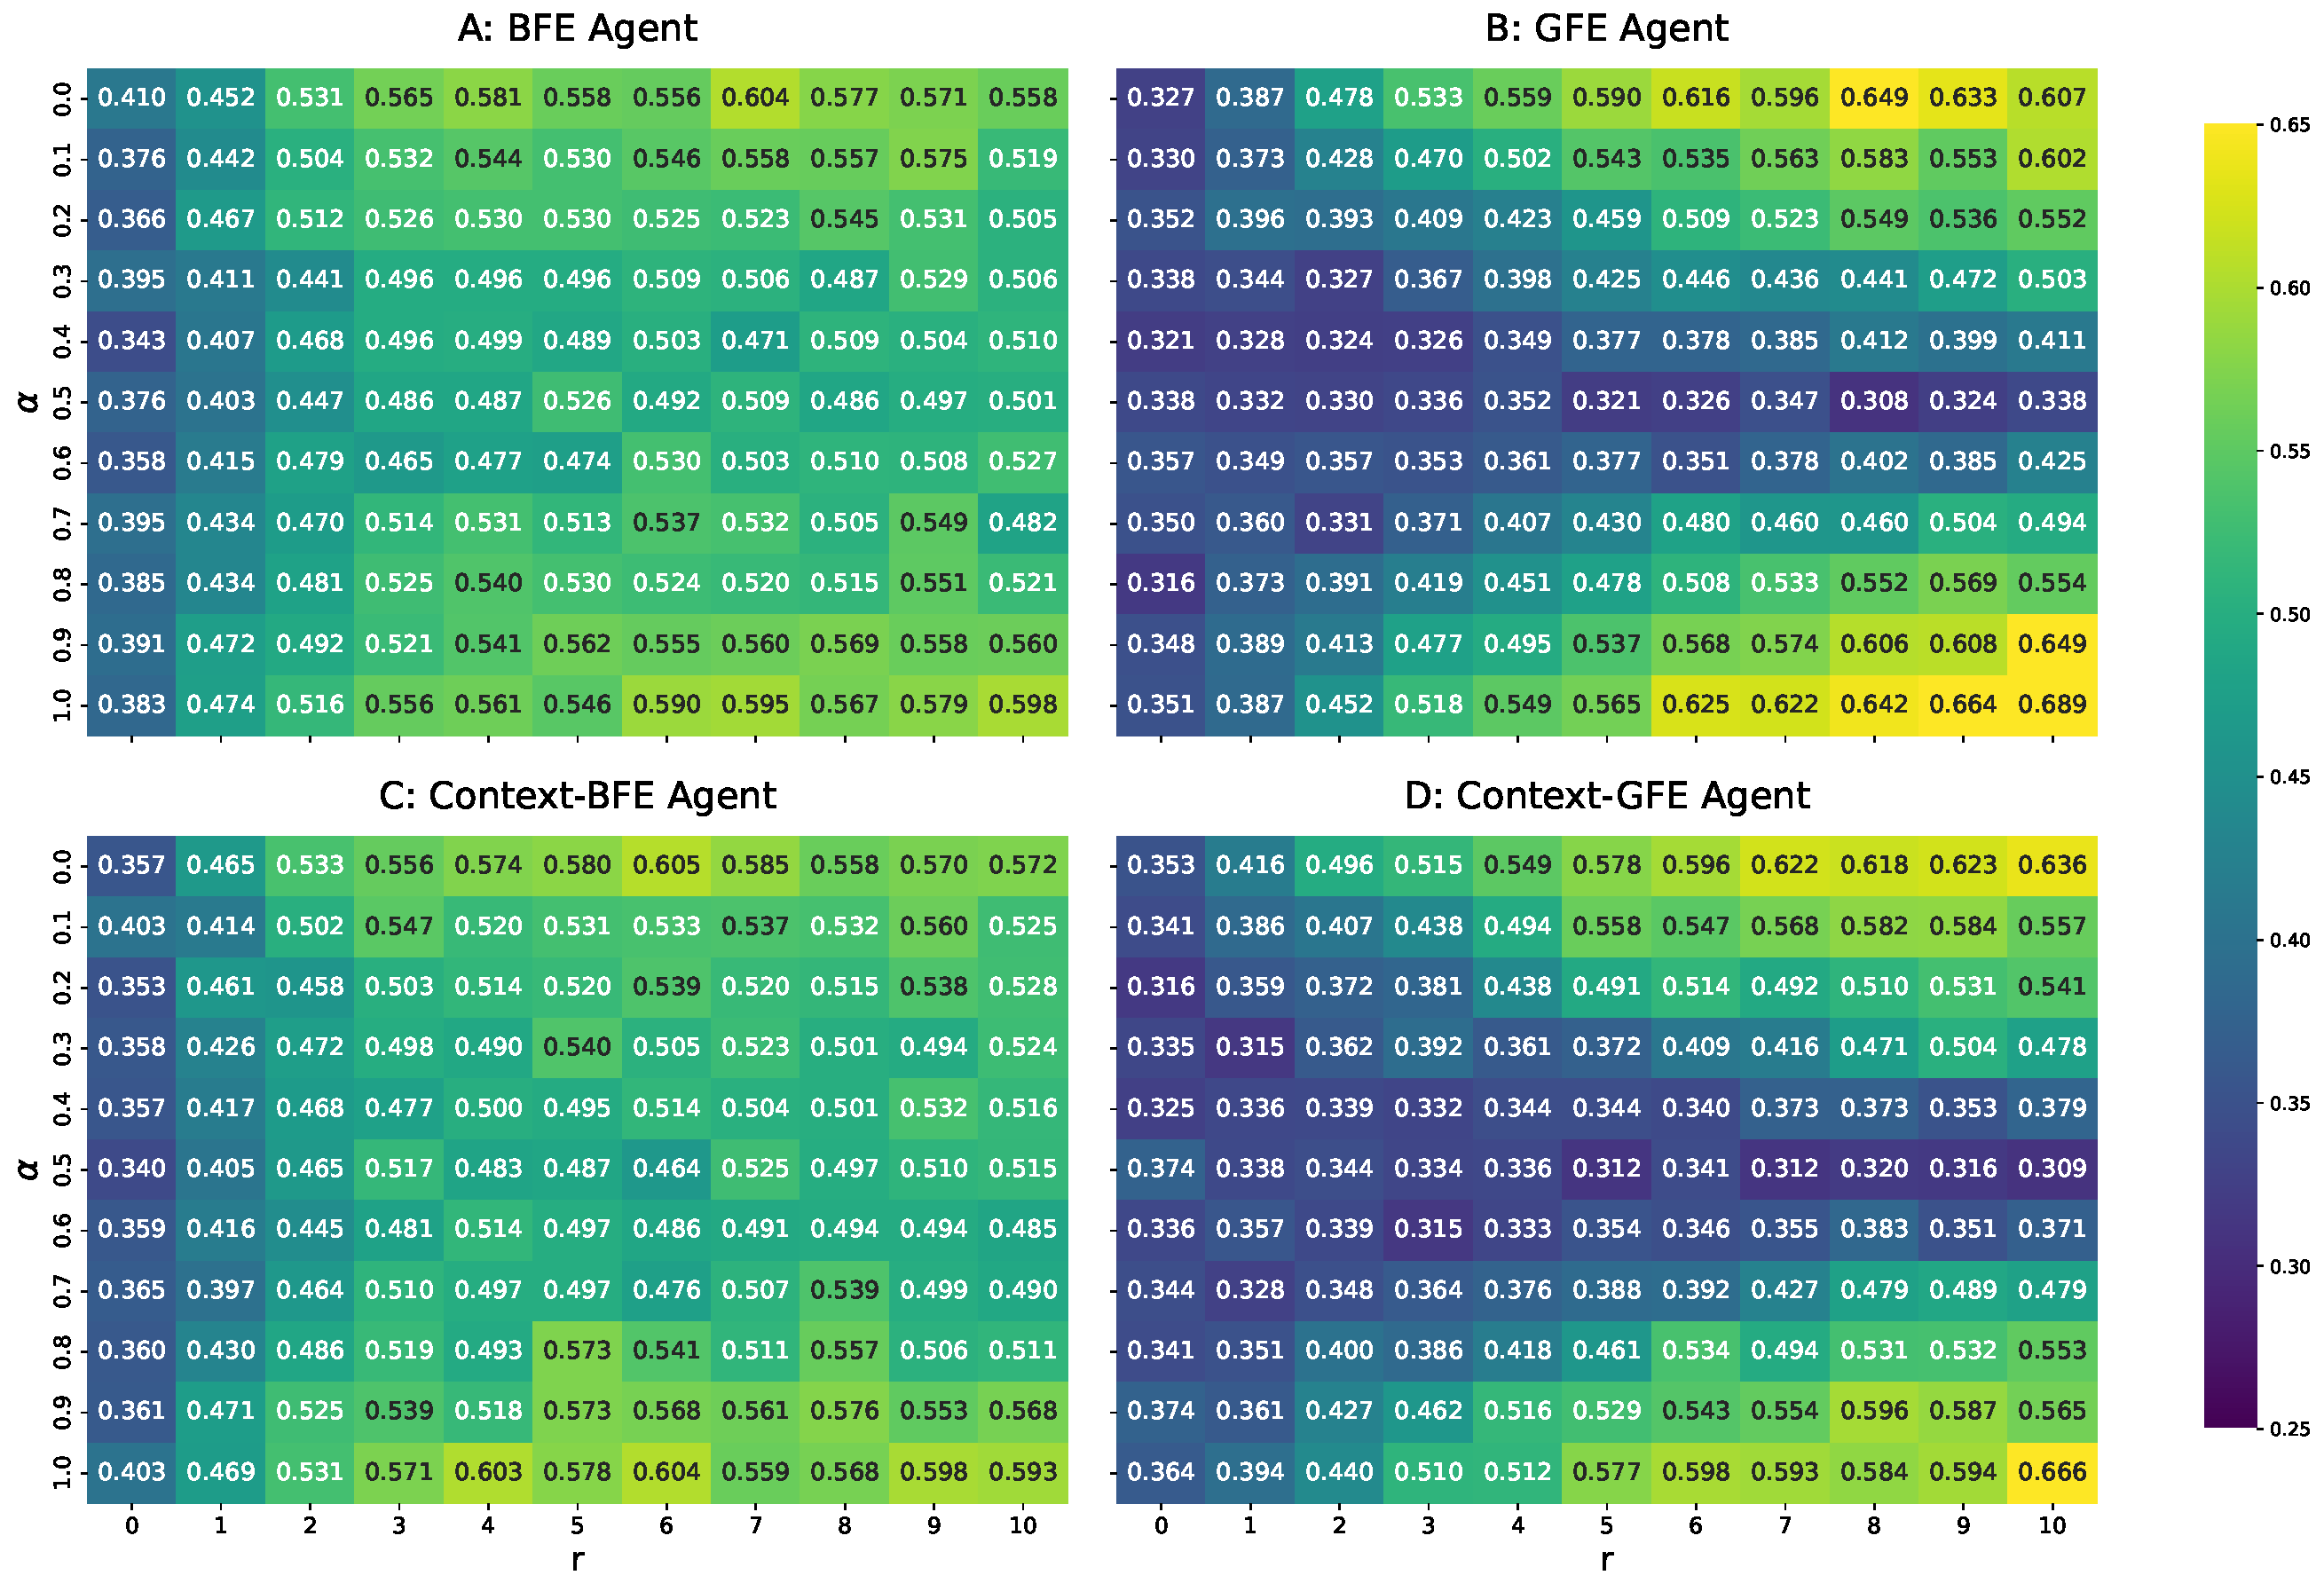
\includegraphics[width=\textwidth]{figures/simulation_3.pdf}
    \caption{Ratios of receiving the reward in timestep \(t=1\) or \(t=2\) over \(1000\) trials for the four agents (BFE, GFE, Context-BFE, and Context-GFE) with differing \(\alpha\)- and \(c\) values.}
    \label{fig:21}
\end{figure}

\subsubsection{Success Factors}

First, I consider the trends that are evident in all four agents. Generally, higher \(c\) values and more extreme \(\alpha\) values lead to higher success rates of receiving the reward in a trial. This is plausible since higher \(c\) values increase the agents' drive of pursuing the reward and more extreme \(\alpha\) values render the cue more useful for moving to the correct arm that contains the reward.

\subsubsection{Curious Agents}

The curious agents appear to have lower success rates for many combinations of \(\alpha\)- and \(c\) values. In these cases their drive of curiousity seem to lead them to alternative behavioral pathways such that they miss out on the reward more regularly.
This situation changes for extreme \(\alpha\)- and high \(c\) values. For these configurations the curious agents receive the reward more regularly than the non-curious agents. In these rare cases, the curious agents "hit" the right balance of going to the cue in the first timestep and being able to use this information in the second step.
